% A Book of Life
% (c) by Brandon CS Sanders, Shelley Sanders, Ben Sibelman,
% Eric Saumur, and other contributing members of The SolSeed Movement
%
%
% A Book of Life is licensed under a
% Creative Commons Attribution-ShareAlike 3.0 Unported License.
%
% You should have received a copy of the license along with this
% work.  If not, see <http://creativecommons.org/licenses/by-sa/3.0/>.
% \documentclass[printer,12pt,openany]{memoir}
\documentclass[ebook,11pt,openany,twoside,draft,showtrims]{memoir}
\usepackage[latin1]{inputenc}
\usepackage{setspace}
\usepackage{tocloft}
\usepackage{graphicx}

\setlength\stockheight {9.25in}% \stockheight=9.25in
\setlength\stockwidth  {6.25in}% \stockwidth=6.25in
\setlength\trimtop     {.125in}
\setlength\trimedge    {.125in}

\begin{document}


%\pagenumbering{}
% Set book title
\title{\textbf{A Book of Life}}
% Include Author name and Copyright holder name
\author{The Contributing Members of The }
\begin{titlingpage}
\maketitle
\end{titlingpage}


% 2nd page, thanks message
%-------------------------------------------------------------------------------
\thanks{Thanks to Octavia Butler for the Earthseed books, to Paul Krafel for
his Seeing Nature and Upward Spiral work, and to Life itself for giving rise to
so many wonderful possibilities.}
\newpage



\pagestyle{plain}
% Not enumerated chapter
%-------------------------------------------------------------------------------
\pagenumbering{Roman}

\chapter*{Preface}

\section*{Happy in the sun}

Several years ago I happened upon a picture whose caption struck a chord in me
that resonates to this day. Our family was in the market to join a community
supported agriculture (CSA) program. As we browsed the websites for the various
CSAs in our area we happened across a picture of some sugar pea sprouts along
with the caption ``happy in the sun!''

``Happy in the sun!'' There was nothing complicated about the image or the
caption. The sprouts were simply being sprouts. And yet, there is something
profound about the phrase ``happy in the sun!'' and the way it was juxtaposed
with those sprouts. Those sprouts were living up to their potential. They were
in some sense ``fully alive,'' the very picture of thriving and flourishing.

If someone were to caption a picture of you with ``happy in the sun,'' what
would that picture contain? What is it that you do that drops you into a state
of flow? What engrosses you to the point that time stops passing and there is
only you immersed in the task in the present moment? What is your happy in the
sun? How do you even go about answering these questions? How do you live the
answers once you have them?

\section*{More or less alive}

There was a time in my life when the most common thing you'd hear from me was a
sigh. Sitting on a couch in our living room every minute or two I'd sigh. Life
was futile, tasteless and bland.

During this time of sighs I was a graduate student in Computer Science at the
University of Rochester. I was working on interesting problems and getting paid
to learn. Two years earlier I had married a woman that I adored and who loved
me too. On the surface it seemed like I should be relishing my life. Yet there
I sat. Sighing on my couch.

This ``sighing'' period of my life lasted for months. When I look back at this
time, I'm struck by how little gumption I had. It took all of my reserves to
meet the minimums. I was doing what was required, and no more. Any moment when
I wasn't acting on some direct obligation was spent in a vegetative funk,
punctuated only by the occasional sigh.

Things suddenly got better when I began treatment for depression. The contrast
was dramatic. I was full of ideas and brimming over with energy to try new
things. In my new state of anti-depressant induced mania, everything I ate was
incredibly tasty. Every new idea I had seemed as if it would change the world.
Each day was full of zest and I charged around inhaling life.

The contrast between these two adjacent periods of my life has made a lasting
impression on how I see the world. I went from a barely alive vegetative fugue
to a frenetic mania that oozed life. I went from sucking the life out of those
who had the misfortune to be in the same room with me, to pumping up those I
encountered and filling them with a sense of new possibilities for their lives.

These back to back periods of stark contrast opened my eyes to how I, the same
person, could be more or less alive at different points in time. Since then
I've noticed that this same thing often happens to me on a day to day basis.
Some days I am powerful, self-expressed, and the world brims with opportunity.
Other days I am weak, stifled, and trapped in a dead-end life.

This phenomenon of more or less life is not limited to individuals. I noticed
the same dynamic at an internet startup that I worked at for a number of years.
Now it was not just an individual who was more or less alive depending upon the
day, but a company composed of many individuals.

Have you experienced the same phenomenon in your own life? Do you remember a
time when you were working with a group and the experience was fun and playful
--- full of life. Ideas came easy and everyone seemed full of energy to carry
them out. Compare that with a meeting during which someone kills the energy in
the group with a mean-spirited comment.

We're used to thinking of life as a binary property. Plants and animals are
alive until they die. But maybe it makes more sense to think of life as a
continuous property. An individual organism, a group of organisms, and indeed
the body of all life can be more or less alive from moment to moment.

This book describes the SolSeed movement, a journey in progress to become fully
alive as individuals, communities, and indeed as the ``body of all life.'' I
hope you find something in it that helps you on your journey!

Bring Life!

Brandon CS Sanders, February 2012


% If the chapter ends in an odd page, you may want to skip having the page
%  number in the empty page
\newpage
\thispagestyle{empty}
\pagenumbering{arabic}
\part{A Vision for Life}

\newpage
\pagestyle{plain}

% First enumerated chapter
%-------------------------------------------------------------------------------
\chapter{Life \ldots it's our epic story!}

\section*{Life is worthy of veneration}

% [[Image:Leafcutter_ant_carrying_leaf.jpg|400px]]

\begin{quote}
{\em The beauty of a living thing is not the atoms that go into it, but the way
those atoms are put together. --Carl Sagan}
\end{quote}

Life puts atoms together in very interesting ways. One configuration of atoms
gives us an ant carrying a leaf many times larger than itself. From another
configuration we get an eagle slipping gracefully through the sky. Yet another
configuration becomes a person who feels, thinks, and loves.

Without Life, the energy from our sun simply bounces off the planet. Life
literally collects the energy Sol sends to earth, and stores it up for future
use. Plants take energy from Sol and convert it into denser, more storable
forms. The sugars and fats that our bodies burn are little pools of energy that
originally came from our sun.

Ants carrying, eagles soaring, people loving \ldots none of these would exist
without Life's awesome capacity for organizing matter.

\section*{Worthy, but not perfect}

% [[Image:WhatIsWorthy.jpg|400px]]
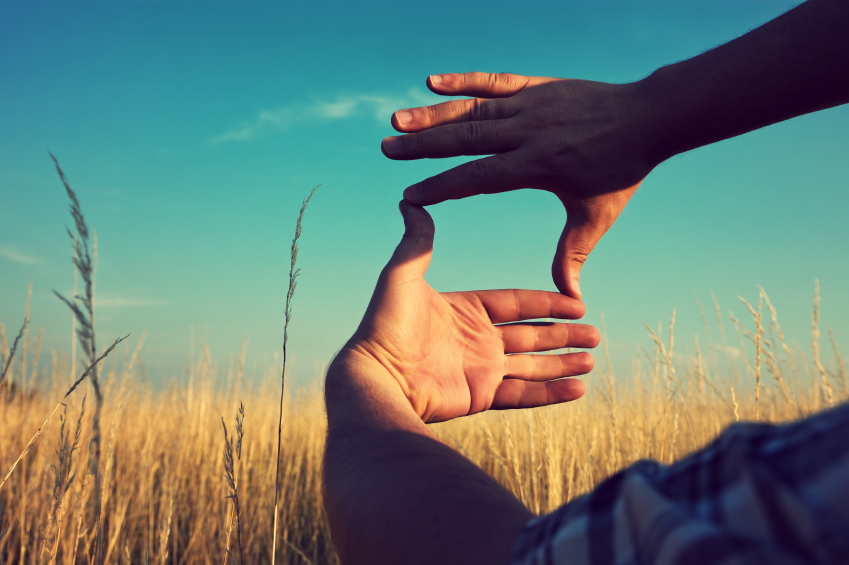
\includegraphics[keepaspectratio=true, width=300px]{images/WhatIsWorthy}

Life is not perfect. This is obvious to anyone who has experienced cruelty or
misfortune. And yet, Life is the only game in town. Without Life the Earth
would be just another dead ball of rock.

Life cannot exist without death. This means that the alternative to death is
the absence of Life. Imagine that everything that had ever lived was still
alive today. There is not space on the earth for all those creatures. The only
way there could be space for them all is if at some point in time they had
stopped reproducing altogether. But reproduction is what powers evolution.
Without reproduction there would be nothing but simple primordial slime, barely
metabolizing in a stagnant stinking sea. But not to worry, there would be
no-one to complain about the smell.

Life is also intrinsically messy. There is in the wake of every living organism
a stream of refuse. In the words of Paul Krafel, consuming things we need and
dumping our waste is an ancient and venerable part of Life. Consumption and
dumping is an essential part of Life. And yet there is more to Life than just
consumption and dumping. Life also creates the conditions for more Life in an
upward spiral of ever greater possibilities. In addition to the get mine
attitude it is also possible to cultivate a grow ours attitude. It is also
possible to practice a way of living that considers the needs of others as if
they were our own.

Life is what it is \ldots and it is worthy of veneration!

\section*{Destruction is Quick and Easy}

% [[Image:Rotting_Collapsing_House.jpg|400px]]

Every one of us knows from personal experience that it is easier to destroy
things than it is to create them. In fact, we don't even need to exert
ourselves to destroy things. If we just ignore them for a while they will erode
and disappear. A vacant house that starts out structurally sound quickly rots
into a sagging derelict \ldots unsafe for human occupation.

In the opening scene of his movie, The Upward Spiral, Paul Krafel contrasts two
different scenarios in which a tower of blocks rises from the ground. The same
two boys create the tower in both sequences. In the first sequence the boys
slowly build the tower one block at a time. In the second sequence the boys
simply raise their hands up from the ground and the tower springs up in their
wake. The building of the tower in the second sequence looks like an explosion
of blocks placing themselves one on top of the other in a trail of creation
following the movement of the boys' hands.

The two videos of the tower being built demonstrate the assymetry between
creation and destruction. If you reverse the video of the boys building the
tower you see them slowly dismantling it, one block at a time. This slow
dismantling doesn't violate our reality detectors. It may be a little out of
the ordinary, after all they could have just knocked the tower down and been
done with it. But we can imagine the boys patiently taking the tower apart one
block at a time.

The second video of the tower exploding into existence is clearly a fake. We
know that no matter how sophisticated the boys are, the world simply does not
work that way. If we reverse the second video we see two boys knocking a tower
down by moving their hands from the top of the tower down to the ground. The
explosion of destruction lines up with our experience and we suddenly
understand the nature of the fakery in the video. The boys actually destroyed
the tower and the filmmaker played it backward to mess with us!

Building a tower of blocks requires sophisticated coordination patiently
deployed over time. Destroying the tower needs only the clumsiest of efforts
requiring neither care nor patience. It is easier to destroy than to create.
The destruction of possibility is the natural order of things. Scientists call
this tendency for things to run down the ``second law of thermodynamics.'' The
second law can be summarized as ``energy always flows downhill toward less and
less usable forms.''

And yet many wondrously complex things do exist! In our world that is strongly
biased towards decay and collapse, how is this possible?

\section*{The upward spiral of life}

% [[Image:UpwardSpiral.jpg|400px]]

\newcommand{\tab}{\hspace*{2em}}

\indentpattern{01}
\begin{verse}
\begin{patverse}
\em
Life creates the conditions for more Life,\\
in an Upward Spiral of ever-growing possibilities.\\
\end{patverse}
\end{verse}

Life is the force that creates an upward eddy in the downward current of
destruction. Creation by life is a process of slow growth. The laying down of
one layer on top of another. This slow process of creation often spans
generations.

Turning to Paul Krafel's ``The Upward Spiral'' again, we find succession as
more than just a brutal competition in which taller plants shade out shorter
plants. In fact, the shorter plants that came first created the conditions that
allowed the taller plants to exist at all. The story is about competition, but
it is not just about competition. It is also a story of multi-generational,
multi-species cooperation to slowly raise up greater and greater possibilities.

The process of evolution that created the wonderful diversity of species is a
long slow steady climb. And like the story of succession, it is a story of
competition AND a story of cooperation. The long slow steady climb of evolution
is the story of the creation of possibilities by countless individuals making
countless contributions across countless generations.

Ants carrying, eagles soaring, people loving \ldots none of these would exist
without Life's slow and steady creation. Life creates an upward spiral of
ever-growing possibilities! And we are agents of Life!

Wherever we go, whatever we do, our sacred duty is to bring Life with us. As we
pursue the work of Life, we must create around ourselves the conditions that
support us being fully alive, that help us flourish and thrive ``Happy in the
sun!'' When we walk into a room full of other people, our task is to increase
the freedom, expression, and possibility those people feel --- to help the
group itself flourish and thrive ``Happy in the sun!'' As we live in our local
and global ecosystem, our charge is to give back more than we take --- to help
the body of all Life also flourish and thrive ``Happy in the sun!''

\section*{The Ultimate Fate of the Universe}

In our vast empty universe, things are running down. The second law of
thermodynamics tells us that possibility will gradually diminish until the
entire universe is nearly the same lukewarm temperature and there are only the
weakest energy gradients to drive the flows of matter and energy that make life
possible. Taking the universe as a whole, this arrow toward decreasing
complexity and opportunity seems to be an absolute. Things ARE running down.
This effect is called entropy and the future it predicts is called the Big
Freeze.

And yet, there is another arrow that points back upstream. This second arrow is
in the direction of life. In the cosmic perspective that encompasses all time
and space, this arrow of life is simply an eddy in a vast current streaming
toward the heat death of the universe. But this eddy, this upward spiral of
life, is the most precious thing in all existence. This effect is called
emergence and the future it predicts does not have a name.

Life has the potential to last an infinite amount of time. Although energy
gradients are ever decreasing they will never completely run out. Life adapts
to changing conditions through evolution. Dr. Freeman Dyson of Princeton
University has demonstrated that life can actually rejoice in an infinite
subjective experience with an infinite amount of time but a finite amount of
energy. (Dyson, Freeman, 1988, Infinite in All Directions page 111)

But Dr. Dyson wrote this before the discovery of dark energy. Dark energy poses
a dangerous threat to our distance future. Physicists have found that dark
energy is increasing in power. They have not measured how quickly it is
increasing yet but if it is increasing quickly enough then it will outpace
entropy and eventually destroy the universe, tearing first galaxies, then
stars, then planets and finally even people apart? This possible future is
called the Big Rip.

How are we to be ``happy in the sun'' when we are caught between these two
possible futures, the Big Rip and the Big Freeze? It is a frightening future
that physicists paint. But we know very little about dark energy yet. The Big
Rip, if it is coming is billions of years in the future. Is it possible for
life to harness dark energy? In billions of years life can learn to grow on
dark energy, and life can grow exponentially outpacing the growth of dark
energy. Perhaps, in the distance future, life can learn to balance dark energy
and entropy, growing ever more complex and creating ever more possibilities,
using enough dark energy to prevent the Big Rip and leaving enough to prevent
the Big Freeze.

Physicists prefer to look at the universe as a dead mechanism in which life is
but an observer. But it was physicists themselves who discovered that it is
impossible to observe without changing what is observed. It may be life's
destiny to control the fate of the universe and our destiny to help life take a
crucial step toward its destiny.

\section*{The ``body of all life''}

\begin{quote}
\em
The beauty of a living thing is not just in the atoms that go into it but in
the way those atoms are put together. --Carl Sagan
\end{quote}

The cells in your body don't know who you are and don't care about you. And
yet, by each cell doing its own little thing in its own little context, this
miraculous emergent thing called you happens!

Groups of people are more than the sum of the individual parts just as the
group of cells in our body is more than the sum of the individual parts. When a
group of people are talking together they will have ideas and think about
things in a way that is different from what the individuals alone would come up
with. To paraphrase Sagan the beauty of an effective team is not just in the
living beings that go into it but in the way those living beings interact
together.

Just like our body is composed of cells that each do their own different unique
thing, so too there is a body of all life composed of living organisms of which
we are a part. What stage of development is the body of all life in right now?
Is it an infant that is yet to become self aware? Or at the other extreme, is
the body of all life already senile and decrepit?

In the cosmic scale of time, conscious life is still very young. As a body of
all life we're probably not even school aged yet. Imagining a human trajectory
for the body of all life we expect the growth through childhood and adolescence
to be attended by a growth in opportunities. The possibilities grow along with
us. As we reach adulthood, we begin to make focused investments toward
particular callings. As we focus and invest in particular areas, some
opportunities that we chose not to focus on become unavailable.

Imagine for a moment that the body of all life is your child. What investments
has your child made in its future? What opportunities lie within arms length?
Given who the body of all life is right now, what do you want for your child in
the future?

{
\em
juxtapose a homeless man or woman who's gone to drink against a happy family
that is healthy and thriving in the sun.

Put together an art exhibition or some sort of creative thing that shows all
kind of different visions for the future of the body of life.

SolSeed imagines the future for the body of all life becoming not just a lone
individual world, but a family of living worlds with great diverse opportunity
among them for what life can become. Each world perhaps specializing in the
family. This world no longer alone in the universe.
}

\section*{Life has invested in us}

% [[Image:ViolinMaker.jpg|400px]]

\begin{quote}
	\em
Every item has its use, a role to play, a thing to do. \\
\tab \tab --From a SolSeed children's song
\end{quote}

Getting a good return of investment (ROI) depends upon making good use of the
thing you've invested in. If you invest in a fine Stradivarius violin, you are
tying up resources in the violin that could have been used on a different
investment. To get a good return from the violin you use it to play beautiful
music. If you want to be sure that the investment in the violin is a total
waste, you use it to pound in nails. The violin makes a lousy hammer and its
ability to produce beautiful music is destroyed by encounters with the nails.

Life is a lot like a human investor charged to manage a large fund. The
``fund'' that Life manages is the pool of diversity and other accumulated
resources of our biosphere. Just like a human investor, Life risks resources on
bets that may or may not provide a good rate of return. Good bets increase
diversity and possibility, bad bets do the opposite.

Right now, Life has a lot riding on humanity. Consider the myriad species that
have gone or will go extinct as a result of human activity. Consider also the
human consumption of fossil fuels, a large portion of Life's densest reserves
of concentrated energy. We're using up pools of energy that took eons to
accumulate. These are significant expenses. What can humanity do that provides
Life with a good ROI on its investment in us? What is it that humanity can do
for Life that is unique? Has all the expense been squandered on consumption? Or
have those extinct species and precious fossil fuels purchased an
infrastructure that could be of use to Life?

Investment is one metaphor. Paul Krafel, a teacher, has a different way of
looking at this story:

\begin{quote}
	\em
	``We are in a very dangerous part of a necessary learning curve. By
degrading our environment, we are learning that we have the power to change it.
Now we can begin to wonder what change in the other (harder) direction would
look like. Now we can begin to practice patience, perseverence, and
self-restraint. We can learn to listen and watch. If we can learn quickly
enough, our current destruction of other species and habitats contains within
it a seed of hope.''

\tab \tab Seeing Nature, p. 170
\end{quote}

The metaphor of learning and the metaphor of investment can be combined.
Perhaps humanity has just realized that its education, the long project of
scientists seeking knowledge by studying the world around us and engineers
using that knowledge to build useful things, was not free. Without realizing
it, we've taken out a gigantic student loan from the Bank of Gaia, and the
interest is now piling up. If we default on our debt, both debtor and creditor
will suffer immensely. But by paying it back in the form of works that help
ecosystems thrive (after first learning how to do those works properly), we can
both provide just compensation to the Bank of Gaia for all the trouble we've
caused, and ensure that it will still be willing to lend resources to us in the
future.

\section*{Who you are}

% [[Image:RayOfSummerSun.jpg|400px]]

\begin{verse}
\em
Ray of summer sun\\
Inseparable from Sol\\
Know yourself and thrive.
\end{verse}

Einstein as he developed the theory of relativity often imagined what it would
be like to ride alongside a beam of light. I invite you to do something
similar. Imagine yourself actually as a beam of light. A ray of sunshine from
our star whose name is Sol. As this sunbeam, you have several different ways
that you can think of yourself. On the one hand you are a transient burst of
photons that will soon be absorbed and cease to exist. On the other hand you
are the Sun itself. You are the provider of practically all the energy that
animates life on earth.

The ability to sometimes perceive ourselves not just as the ephemeral ray of
light, but as the sun itself can add a great deal of power and purpose to our
lives. This ability to identify with the larger whole is an essential
characteristic of spiritual enlightenment. It offers freedom from reactive
grasping and the option to proactively create our lives.

I invite you to take a moment to close your eyes and imagine that you are not
just your skin-bag, but that you are life itself! Think of the possibilities!

Excesses of the non-dual perspective

Inadequacies of the simply dualistic perspective. Anxiety paralysis
self-loathing fear -reactive rather than proactive.


\section*{Your calling}
% <youtube>8g4d-rnhuSg</youtube>

Living a beautiful life

It's naive to think that there is only one job one role that each person can
play. Thinking of this way leads us to spend our entire lives searching for who
we are and what our job is. Perfect is the enemy of good enough and right now.
living a perfect life is impossible our goal should instead be to live a
beautiful life. Is there one perfect painting one perfect meal? No! There are
many great meals many great paintings and there are also many lousy meals and
many lousy paintings.


\begin{quote}
\em
Our obligation to survive and flourish is owed not just to ourselves but also
to that Cosmos ancient and vast from which we spring. --Carl Sagan
\end{quote}

The history of life is a many branching tree and humanity is just one branch on
that tree. When inhabitants of the far future look back on humanity as it is
now, they will see not the pinnacle of evolution, but a transitional species
that diverged into new branches in the tree of life. Our place in the body of
all life is not one of special rights and privileges, but rather one of purpose
and responsibility. As life's intelligent spark we are called to nurture the
body of all life -- we are called to ensure that it survives and flourishes.

We are called not just to live -- not just to get by -- but to create a life
that brings honor to all the ancestors who came before us and creates
opportunities for all the generations that will follow us.

Borrowing a metaphor from Erwin Ramsdell Goodenough:

\begin{quote}
	\em Life is a coral reef. We each leave behind the best, the strongest
	deposit we can so that the reef can grow. But what's important is the
	reef.
\end{quote}


% Last pages for ToC
%-------------------------------------------------------------------------------
\newpage
% Include dots between chapter name and page number
%Finally, include the ToC
\tableofcontents




\end{document}
